
\section{Un exemple de codage : le jeu de Nim}
\subsection{Description du jeu de Nim}

Le principe du \game est le suivant : on dispose au départ d'un nombre $\nbAllumettes$ non nul d'allumettes
% IL EST IMPORTANT DE SPECIFIER QUE LE NB D'ALLUMETTES EST NON NUL CAR NOTRE DEF DE 0_PERD NE DEFINIT CETTE NOTION QUE POUR t>0 !!!
et un nombre $\nbJoueurs$ de joueurs peuvent prendre $1$ ou plusieurs allumette(s). Le joueur qui perd est celui qui, le premier, ne peut plus prendre d'allumette.\footnote{Il existe différentes variantes de ce jeu, notamment en faisant varier les nombres d'allumettes et de joueurs, mais également en faisant varier les actions possibles ou en introduisant des contraintes (par exemple, on ne peut pas prendre le même nombre d'allumettes que le joueur précédent).} Le nombre de tours de jeu possibles est au plus égal à celui des allumettes (à minima, chaque joueur ne prend à chaque tour qu'une seule allumette). Ainsi, l'ensemble des indices des tours possibles est $\turnsSet = \{ 0, ..., \nbAllumettes \}$ où $0$ est l'indice de l'état initial. De même, l'ensemble des nombres possibles d'allumettes encore disponibles est $\matchesSet = \{ 0, 1, ..., \nbAllumettes \}$.

Afin de simplifier au maximum le langage utilisé, nous modélisons ici une variante où $\nbAllumettes = 4$ et $\nbJoueurs = 2$. Les joueurs sont notés $0$ et $1$ et c'est au tour de $0$ de jouer au tour $t$ ssi $\turn{t}$ est vrai (considérant que si ce n'est pas le tour de $0$ alors c'est celui de $1$). De plus, $\rest{t}{n}$ est vrai ssi au tour $t$ il reste $n$ allumettes.

Ainsi, l'état initial du jeu est le suivant : 
\begin{gather}
\rest{0}{\nbAllumettes} \land \turn{0}
\label{eq:initialState}
\end{gather}
indiquant qu'au tour $0$ il y a encore $\nbAllumettes$ de disponible et que c'est au tour de $0$ de jouer.

Dans la version présentée ici du \game, on limite également le nombre des actions possibles à deux : un joueur peut prendre soit $1$ allumette, soit $2$ allumettes. Ainsi, $\takes{t}$ est vrai ssi un agent prend $2$ allumettes au tour $t$ (considérant ainsi que $\takes{t}$ est faux ssi il n'en prend qu'une). 

Ainsi :
\begin{align}
%\begin{split} TODO
\bigwedge_{\substack{t \in \turnsSet%\\
n \in \matchesSet%\\
n \geq 2}}
    \bigg ( & \Big ( \rest{t}{n} \land \takes{t} \limp%\\
    & \hspace{1.5cm}\rest{t+1}{n-2} \ \Big ) \; \land \\
    & \Big ( \rest{t}{n} \land \neg \takes{t} \limp %\\
    & \hspace{1.5cm}\rest{t+1}{n-1} \Big ) \bigg )
%\end{split}
\end{align}
capture le fait que si au tour $t$ il reste au moins $2$ allumettes et qu'un joueur en prend $2$ alors au tour suivant il en reste $2$ de moins, et que si il n'en prend qu'une alors au tour suivant il en reste $1$ de moins.

En revanche, si au tour $t$ il reste exactement $1$ allumette, alors nécessairement le joueur en prendra $1$ et il en restera $0$ au tour suivant :
\begin{gather}
\bigwedge_{t \in \turnsSet}
    \Big (\rest{t}{1} \limp \neg \takes{t} \land \rest{t+1}{0}\Big )
\end{gather}

Notre modèle spécifie ensuite que :
\begin{align}
& \bigwedge_{t \in \turnsSet}
    \bigvee_{n \in \matchesSet}
        \rest{t}{n} \\
& \bigwedge_{\substack{t \in \turnsSet\\ n1, n2 \in \matchesSet\\ n1 \neq n2}}
    \Big ( \rest{t}{n1} \limp \neg\rest{t}{n2} \Big )
\end{align}
La première formule stipule qu'à chaque tour $t$ il existe au moins un nombre $n$ d'allumettes restant, et la seconde que ce nombre est unique.

\begin{figure*}
\centering
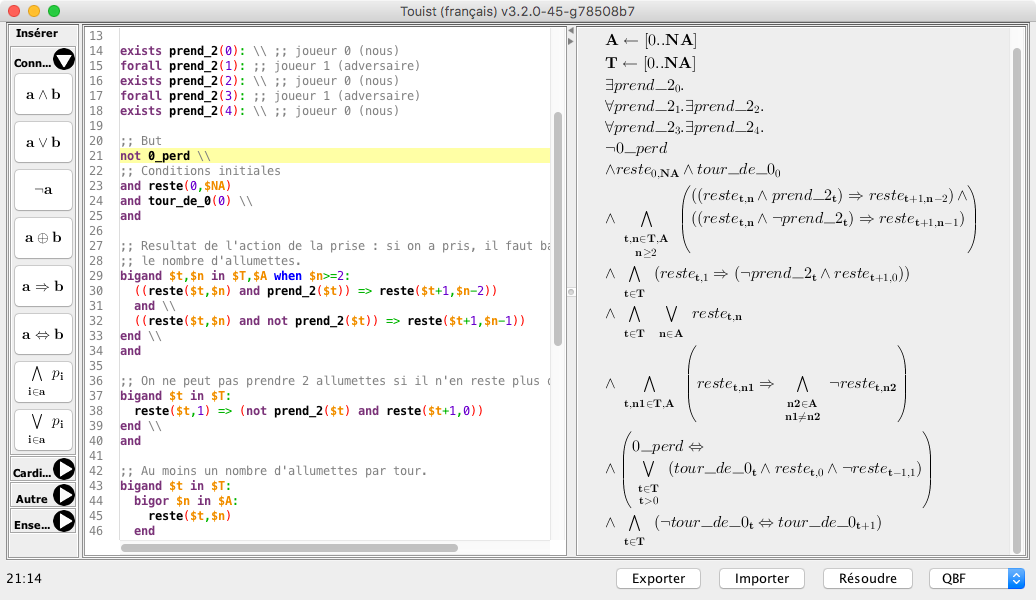
\includegraphics[width=0.9\textwidth]{figures/touistScreenshot}
\caption{Capture d'écran de \touist avec le \game. Le fichier est disponible à l'adresse \url{https://github.com/maelvalais/allumettes}}
\label{fig:touistScreenshot}
\end{figure*}

Il faut maintenant définir quand un joueur a perdu :
\begin{gather}
\begin{split}
\lost \lequiv \bigvee_{\substack{t \in \turnsSet\\ t > 0}} & \bigg ( \turn{t} \land \rest{t}{0} %\land \\
%    &  \Big ( \rest{t-1}{1} \lor \rest{t-1}{2} \Big 
\bigg )
\end{split}
\end{gather}
signifie que le joueur $0$ a perdu ssi il existe un tour $t$ où il reste $0$ allumettes alors qu'à l'instant d'avant il y en avait au moins une.

Finalement, à chaque tour $t$, ce n'est pas au joueur $0$ de jouer ssi c'est à lui de jouer au tour suivant :
\begin{gather}
\bigwedge_{t \in \turnsSet \setminus \{ \nbAllumettes \} } \Big (
    \neg \turn{t} \lequiv \turn{t+1}
\Big )
\label{eq:turnChange}
\end{gather}



\subsection{Formalisation d'une stratégie gagnante à l'aide de QBF}

Dans cette section, nous allons présenter à l'aide de notre exemple du \game l'extension de \touist à QBF.

Le langage de QBF permet d'exprimer naturellement et de manière concise l'existence de stratégies gagnantes ainsi que décrit dans \cite{DBLP:series/txtcs/KroeningS16}. Les coups du joueur 0 (pour lequel on cherche une stratégie gagnante) seront existentiellement quantifiés alors que ceux de son adversaire seront universellement quantifiés. (On cherche les coups du joueur $0$ qui le mèneront à la victoire quels que soient les coups joués par le joueur $1$.)

\touist a été étendu pour être compatible avec le solveur QBF \emph{Quantor 3.2} \cite{Biere:2004:RE:2103144.2103150}. La sélection de ce prouveur dans \touist autorise \emph{de facto} l'utilisation des quantificateurs $\forall$ et $\exists$ (respectivement définis par \verb+exists+ et \verb+forall+ dans \touist).

\begin{figure}
\centering
\tikzset{%
    prend1/.style={->,dotted,very thick,>=latex},
    prend2/.style={->,very thick,>=latex}%
}

\begin{tikzpicture}
% définition des noeuds
\node (t0) at (0.5,0) {4};
\node (t11) at (-1,-1) {2};
\node (t12) at (2,-1) {3};
\node (t21) at (-2,-2) {0};
\node (t22) at (0,-2) {1};
\node (t23) at (1,-2) {1};
\node (t24) at (3,-2) {2};
\node (t31) at (0,-3) {0};
\node (t32) at (1,-3) {0};
\node (t33) at (2,-3) {0};
\node (t34) at (4,-3) {1};
\node (t4) at (4,-4) {0};
% 0 joue
\draw[prend2] (t0)--(t11);
\draw[color=red][prend1] (t0)--(t12);
% 1 joue
\draw[prend2] (t11)--(t21);
\draw[prend1] (t11)--(t22);
\draw[color=red][prend2] (t12)--(t23);
\draw[color=red][prend1] (t12)--(t24);
% 0 joue
\draw[prend1] (t22)--(t31);
\draw[color=red][prend1] (t23)--(t32);
\draw[color=red][prend2] (t24)--(t33);
\draw[prend1] (t24)--(t34);
% 1 joue
\draw[prend1] (t34)--(t4);
\end{tikzpicture}

\caption{Solutions pour le \game (4 all./2 joueurs), en rouge : stratégie gagnante du joueur 0}
\label{fig:solutions}
\vspace{-0.5cm}\end{figure}

\tikzset{%
    prend1/.style={->,dotted,very thick,>=latex},
    prend2/.style={->,very thick,>=latex}%
}


\figurename~\ref{fig:solutions} présente l'ensemble exhaustif des solutions de notre exemple. La racine de l'arbre représente le nombre initial d'allumettes, et chaque flèche l'action de retirer $1$ (\tikz{\draw[prend1] (0,0) -- (1,0)}) ou $2$ (\tikz{\draw[prend2] (0,0) -- (1,0)}) allumette(s). Au bout de la flèche, le nombre d'allumettes après exécution de l'action concernée. D'après cette figure, on voit que si le joueur $0$ commence (ce qui est imposé par (\ref{eq:initialState})) et qu'il retire une seule allumette (il en reste donc 3) on voit qu'il a une stratégie gagnante : 
\begin{itemize}
\item si le joueur $1$ retire ensuite $2$ allumettes il en restera $1$ seule que le joueur $0$ peut retirer pour gagner (puisque le joueur $1$ ne pourra ensuite plus retirer d'allumette) ;

\item si le joueur $1$ retire une seule allumette, il en restera  $2$ et le joueur $0$ pourra au coup suivant les retirer en un seul coup et le joueur $1$ perd.
\end{itemize}

Nous tirons parti de QBF pour écrire cette stratégie dans \touist. Si on note $\Phi$ la conjonction des formules (\ref{eq:initialState}) à (\ref{eq:turnChange}) alors la recherche d'une stratégie gagnante pour le joueur $0$ s'écrit simplement :
\vspace{-0.2cm}
\begin{align}
\begin{split}
&\exists \takes{0}
\forall \takes{1}\\
&\qquad\exists \takes{2}
\forall \takes{3} \\
&\quad\exists \takes{4}\text{ . }\neg \lost \land \Phi
\end{split}
\end{align}

\noindent
Autrement dit, on cherche à satisfaire le fait qu'il existe une action du joueur $0$ au tour $0$ telle que quelle que soit l'action du joueur $1$ au tour $1$, il existe une action du joueur $0$ au tour $2$, telle que pour toute action du joueur $1$ au tour $3$ il existe une action du joueur $0$ (qui sera donc le dernier à jouer) telle que le joueur $0$ ne perd pas et que les contraintes inhérentes au \game soient satisfaites.

% \warning{[DOMI : ] Je ne suis pas sûr de ce qui suit car je n'arrive pas à faire fonctionner le prog des allumettes avec la dernière version de \touist (ça plante).}

L'exécution du programme dans \touist indique que cette formule est vraie, ce qui signifie l'existence d'une stratégie gagnante pour le joueur $0$. Le solveur retourne la valeur des (ici une seule) variables existentielles correspondant au prochain coup du joueur $0$. À ce stade, le joueur adverse doit fournir son coup qui fixe la valeur des variables universelles correspondant à ses possibles prochains coups. On exécute alors de nouveau le programme modifié de la façon suivante (de manière à prendre en compte le calcul de la valuation de $\takes{0}$) :
\begin{align*}
\begin{split}
&\exists \takes{0}
\exists \takes{1}\\
&\qquad\exists \takes{2}
\forall \takes{3} \\
&\quad\exists \takes{4}\text{ . }\neg \lost \land c_0 \land c_1 \land  \Phi
\end{split}
\end{align*}
où $c_0$ est soit $\takes{0}$ soit $\neg \takes{0}$ en fonction du coup du joueur $0$, et similairement pour $c_1$ en fonction du coup choisi par l'adversaire. La  situation après ces deux coups est la nouvelle situation initiale pour le solveur et la recherche du coup suivant du joueur $0$... jusqu'à sa victoire ! On réitère ce processus jusqu'à ce que toutes les variables aient reçu une valeur. 
%On obtient alors :
%\begin{gather*}
%\interpret[\takes{0}] = 0, 
%\interpret[\takes{1}] = 1 
%\interpret[\takes{2}] = 0
%\end{gather*}
%qui se lit : pour que le joueur $0$ gagne il doit prendre $1$ allumette, le joueur $1$ en prend $2$, puis le joueur $0$ en prend $1$.